
% introduce: why only  consider point-edge contact

\section{Automated design of peg and socket}


In this section, we introduce an automated design process to fine-tune the peg and socket design in 2D, so that the resulting peg can be successfully inserted into the socket while being most stable after insertion, with respect to the rotation angle of the peg. For a fixed number of contact points on the peg and a fixed number of edges in the socket, the design process iteratively optimize the placement of contact points along the respected contacting socket edge, and the angle of the socket edge. Then, by comparing the design for different number of contact points and the socket edges, we can find the {\em best} design for a pair of peg and socket. 

The iterative optimization process can be briefly described as follows. Given a fixed number of $m$ contact points on the peg and $n$ edges in the socket, we will generate a graph representing all the possible mode of contacts, i.e. how points on the peg may contact different edges of the socket, and how those different mode of contacts may change under a given insertion direction (line of force). The mode of contacts combined with the change of the modes forms a graph, which we refer to as the {\em Contact-Mode Transition Graph} (CMT graph). Once the graph is found, we will find the boundary condition when the transition among the different modes may break with respect to the angle of each edge on the socket. At the same time, we also analyze how rotation angle of the inserted peg may change the contact points on the peg is moved along the respectively contacting edge. Then, we iteratively move the contact point locations and the edge angles to reduce the possible rotation angle for a inserted peg to improve its stability. The output design will be compared with the outcomes for a different number of $m$ and $n$, and the best design will be the final output of the process. 

The following subsections introduce the details of each step of the above process. We will show examples of the intermediate outcomes of the design and compare them in the next section, to demonstrate the correctness of this design process. 


\subsection{Mode of contacts and transitions}

The insertion process of the peg into the socket may involve the points on the peg contacting different edges of the socket at different {\em stages} of the insertion, The goal for the insertion is clear: the peg must be fully inserted into the the socket so that if there is no error in the manufacturing, each point on the peg should contact the designed edge on the socket, even when the initial insertion angle and placement may contain bounded error. 

However, as each contact between a point on the peg and an edge on the socket introduces an additional constraint, the straight optimization of the socket and peg design may involve different set of constraints at different stage of the insertion. The result of the optimization under any given set of constraints may not extend to other stages. We need to find how the effect of the design changes may affect across different stages of the insertion. 

We discretize the insertion process based on different {\em Mode of Contacts}, i.e. a collection of point-edge pairs that are in contact respectively. We refer to each point-edge pair that is contact as a {\em Contact Pair}, denoted as $CP(i, j) = \{p_i, e_j\}$, where $p_i$ is the $i$th point on the peg counter-clockwise, and the $e_j$ is the $j$th edge on the socket counter-clockwise. We also denote the Mode of Contact as $MoC(k) = \{CP(a, b), CP(c, d), \ldots\}$. Then, the entire insertion process can be described as a directed graph when the insertion is guided by any known force. 

In this paper, we only consider the Contact-Pair as the pair containing a point on a peg and an edge on the socket. For simplicity, the points on the peg can be joined by different designs (curves) to avoid any contact between the socket edges other than the bounded number of designed contact points. In addition, a point on the peg contacting two adjacent edges on the socket, i.e., a point-point contact, can be viewed as two contact pairs. Therefore, the Contact-Pair defined above is the fundamental unit for analyzing the Mode of Contact in the peg-socket relation. 


In order to analyze the insertion process and discretize the insertion based on different stages (MoCs), we need to find all valid Mode of Contacts. For a Mode of Contact to be valid, all the containing Contact Pairs should be valid for the given peg and socket, and there exist a valid configuration for the collection of contact pairs based on the peg and socket geometry. Then, for all the valid Contact Pairs, we can find all possible combinations of the Contact Pairs and test the validity of each combination, and the resulting valid combinations are the valid Mode of Contacts between the given peg and socket geometry. The valid Mode of Contacts can also be found by translating and rotating the peg within the socket, but as the rotations and translations is a continuous process, the approach may be slow and inaccurate though easy to implement. 

The Mode of Contacts along cannot fully describe a insertion process, as the insertion process involves the transition between different modes. To find out whether a transition between two Mode of Contact under a given force is possible, we can find the acceleration direction under the insertion force, and the location of the different Contact Pairs between the two modes. If the acceleration / moving direction can lead to the contact or the removal of the corresponding point-edge pairs, then the transition is valid, otherwise not. 

% for example, ....



In reality, ...

% consider all transition among modes is too complex, and only "adjacent" modes can transite under a given force; so we consider only neighbors. How to define neighbors? and is it correct? 

% Following the above definitions and analysis, we can find a CMT graph, and the insertion process is discretized into different Modes, and each mode consists of a fixed set of point-edge contraints, so that the analysis becomes simpler, as well as optimization. 

% Benefits of discritization, existing methods, 




For any peg-socket joint, we can get limited valid contact pairs. By combining different contact pairs, we can get different contact modes ${cm}=\{{cp}\}$. If the contact mode is valid, we denote the contact mode as a node in graph. Then the directed edge between two nodes ${cm}_1\to{cm}_2$ means the mode ${cm}_1$ can transfer along the edge direction to another mode ${cm}_2$ under the given force. 

To discrete the graph further, the contact mode transition only happens among adjacent modes. Here, we define two contact modes ${cm_i}=\{{cp}\}_i$ and ${cm_j}=\{{cp}\}_j$. If contact points of ${cp}$ in the difference set $\{{cp}\mid {cp}\in{cm_i}\cup{cm_j}, {cp}\notin{cm_i}\cap{cm_j}\}$ are the same, ${cm_i}$ and ${cm_j}$ are defined as adjacent modes. This means the difference of contact pairs in adjacent modes is caused by only one peg point. Totally, adjacent modes are in four cases. 
1. The contact point in one contact pair leaves the contact edge.
2. The same contact point in two contact pairs leaves the two contact edges(point-point).
3. One noncontact peg point contacts one socket edge.
4. One noncontact peg point contact two socket edge(point-point).
Here, case 1 and case 2 are called ${cm}$ decrease. Case 3 and case 4 are called ${cm}$ increase.
These contact point and contact edge which cause ${cm}$ increase an decrease are called target point and target edge. 

For ${cm}$ decrease, if the force on target point makes it leave the target edge, that is, signed distance ${d}$ between target point and target edge increases, this mode transition is valid. 
Similarly, for ${cm}$ increase, if the force on target point makes it closer to the target edge, that is, ${d}$ decreases, this mode transition is also valid. Examples of these two mode transition are shown in Figure * and Figure *.

%begin{figure}
%begin{figure}

Assuming the configuration force ${F}$ is along the peg direction, given friction coefficient $\mu$, then we can get friction force ${F_n}=\mu{F}{sin}\theta$, where $\theta$ is signed angle between configuration force and contact edge. The force between contact pair is ${F_p}={F}{cos}\theta-{F_n}$,  and the force on target point can be caculated as ${F_t}={F}-\sum_{{cp}\in{cm}} {F_p}$. Most directed edges of graph can be obtained by ${F_t}$ and the ${d}$ between adjacent modes. However, there are some spacial adjacent modes below which need separate analysis. 

(a). Point-point case, shown in Figure *. Here, the angular bisector and the  tangent divide the plane into three area. If ${F_t}$ direct to area 1, the contact point would leave two contact edge. Otherwise, it would leave the edge opposite to the direction of ${F_t}$.

%begin{figure}
 
(b). ....

To complete the graph, we also define non-contact mode as a special node.

\subsection{Insertion grediant}

Given a peg-socket joint, we can model the graph as above. The graph discretely show the insertion process. If there is a sink, it means the insertion can get a stable contact mode eventually under the configuration force.

Figure~\ref{fig:insetion_graph} is insertion graph for a random five-point and five-edge peg-socket joint.
Here, there are 46 nodes including 45 contact modes(${cm}_1-{cm}_{45}$) and 1 noncontact modes(${cm}_{46}$). We can get 4 sinks from the graph, e.g, ${cm}_{36}$, ${cm}_{37}$, ${cm}_{41}$, and ${cm}_{42}$, which can be shown in Figure~\ref{fig:5_5_sink}. Where, denote ${cp}$ ${i}-{j}$ as contact pair with peg point ${i}$ on socket edge ${j}$ (peg points and socket edges are both count clockwise numbering ) 
\begin{figure}
\begin{center}
\includegraphics[width=2in]{figures/insertion_graph.png}
\end{center}
\caption{The insertion graph of five-point and five-edge peg-socket joint. }
\label{fig:insetion_graph}
\end{figure}

It's reasonable to have four different sinks, since the initial configuration of peg is uncertain. Here, sink1 and sink4 are desired sinks , while sink2 and sink3 are sinks we want to avoid.

\begin{figure*}
\begin{center}
\begin{subfigure}[t]{0.24\textwidth}
\begin{center}
\includegraphics[height=1.3in]{figures/5_5_sink1.png}
\end{center}
\label{fig:5_5_sink1}
\caption{Sink1. Contact mode with three contact pairs, e.g, ${cp}$ 1-1, ${cp}$ 3-3, ${cp}$ 4-4. }
\end{subfigure}
\begin{subfigure}[t]{0.24\textwidth}
\begin{center}
\includegraphics[height=1.3in]{figures/5_5_sink2.png}
\end{center}
\label{fig:5_5_sink2}
\caption{Sink2. Contact mode with three contact pairs, e.g, ${cp}$ 1-1, ${cp}$ 3-4, ${cp}$ 4-5. }
\end{subfigure}
\begin{subfigure}[t]{0.24\textwidth}
\begin{center}
\includegraphics[height=1.3in]{figures/5_5_sink3.png}
\end{center}
\label{fig:5_5_sink3}
\caption{Sink3. Contact mode with three contact pairs, e.g, ${cp}$ 2-1, ${cp}$ 3-2, ${cp}$ 5-5. }
\end{subfigure}
\begin{subfigure}[t]{0.24\textwidth}
\begin{center}
\includegraphics[height=1.3in]{figures/5_5_sink4.png}
\end{center}
\label{fig:5_5_sink4}
\caption{Sink4. Contact mode with three contact pairs, e.g, ${cp}$ 2-2, ${cp}$ 3-3, ${cp}$ 5-5. }
\end{subfigure}
\end{center}
\label{fig:5_5_sink}
\caption{Sinks of five points peg and five edges socket joint insertion graph. }
\end{figure*}

For each sink, we keep contact pairs and the configuration force direction but ignore the geometry. Then the insertion grediant can be obtained by rotating contact edge. If the force between contact pair with rotated contact edge become zero, it means the rotation angle would break the insertion, therefore getting limit rotation angle of socket edge. By calculating limit rotation angle for insertion break of four sinks as above, we get insertion grediant for the peg-socket joint, that is, the rotation of socket edge, which can be shown in Figure *. Then, for each peg-socket joint, fixing the peg, we can get the limit rotation angle of socket edge that not break the insertion.

%begin{figure}


\subsection{Stability grediant}

The stability is reflected by the maximun rotation angle when peg is in socket. Straight geometry rotation is hard to get maximun rotation angle, let along minimizing the maximum rotation angle. Because rotation pivot is variable. Similarly, we model the peg-in-socket motion process as a graph, by which to get maximun rotation angle of each contact mode.

Different form insertion, to keep peg in socket, we addit a top edge to close the socket. In reality, peg should be attached on block base, which is equivalent to the top edge. This edge would additionally limit the configuration of peg. Therefore, we get differerent contact mode and graph. 
The graph and sink are shown in Figure~\ref{fig:stability_graph} and Figure~\ref{fig:5_5closed_sink} respectively.

\begin{figure}
\begin{center}
\includegraphics[width=2in]{figures/stability_graph.png}
\end{center}
\caption{The motion graph of peg-in-socket joint. }
\label{fig:stability_graph}
\end{figure}

\begin{figure}
\begin{center}
\begin{subfigure}[t]{0.24\textwidth}
\begin{center}
\includegraphics[height=1.3in]{figures/5_5closed_sink1.png}
\end{center}
\label{fig:5_5closed_sink1}
\caption{Sink1. Contact mode with three contact pairs, e.g, ${cp}$ 1-1, ${cp}$ 3-3, ${cp}$ 4-4. }
\end{subfigure}
\begin{subfigure}[t]{0.24\textwidth}
\begin{center}
\includegraphics[height=1.3in]{figures/5_5closed_sink2.png}
\end{center}
\label{fig:5_5closed_sink2}
\caption{Sink2. Contact mode with three contact pairs, e.g, ${cp}$ 2-2, ${cp}$ 3-3, ${cp}$ 5-5. }
\end{subfigure}
\label{fig:5_5closed_sink}
\caption{Sinks of five points peg in closed five edges socket joint motion graph. }
\end{center}
\end{figure}

We can see when the peg get block base, that is, closing the socket, the sink2 in Figure~\ref{fig:5_5closed_sink1} and the sink3 in Figure~\ref{fig:5_5closed_sink2} has disappeared, since the corresponding contact mode is invalid. 

Then, for each contact mode, we keep its contact pairs unchanged but move the contact point on contact edge. Then calculate the configuration of moved peg by its geometry. In this way, the peg has been rotated. Loop over the loation of contact point on contact edge untill break the contact mode. Then the maximum ratation angle of each contact mode can be obtained, by comparing the maximum ratation angle, we can get most unstable contact mode.

There are some troubles about calculating rotation angle of contact mode with three or more contact pairs, since three or more points move may result in violence. The result is depend on specific peg-in-socket joint geometry. However, notice that the contact mode with less or more contact pairs are partially order set. Obviouslly, maximum rotation angle of contact mode is less than that of its partial order elements. Hence, we can ignore contact modes with more than two contact pairs. 

Figure~\ref{fig:5_5rotate.png} shows two most unstable contact mode. To get the grediant of stability, we need to find out the which peg design would reduce the maximum rotation angle. For five-point peg, let third peg point on the mid of third edge of socket (numbering counter clockwise).  Denote ${t}_{i}$ be the ratio of peg edge ${i}$ to socket edge ${i}$, e.g, relative position between point ${i}$ and edge ${i}$ without considering peg-socket joint error. Then we can respectively qualitative analysis the influence of ${t}_1$ and ${t}_4$ on maximum rotation angel of contact mode in Figure~\ref{fig:5_5rotate1.png}, and the influence of ${t}_2$ and ${t}_5$ on maximum rotation angel of contact mode in Figure~\ref{fig:5_5rotate2.png}. As said above, desired peg-socket joint should be symmetrical. So ${t}_1$ and ${t}_5$ should the same, as well as ${t}_2$ and ${t}_4$. Denote ${t}_1$ and ${t}_5$ as ${t}_{up}$, ${t}_2$ and ${t}_4$ as ${t}_{low}$. Then we can get the grediant of stability, e.g, the change of ${t}_{up}$ and ${t}_{low}$.

\begin{figure}
\begin{center}
\begin{subfigure}[t]{0.24\textwidth}
\begin{center}
\includegraphics[height=1.3in]{figures/5_5rotate1.png}
\end{center}
\label{fig:5_5rotate1}
\caption{The rotation of contact mode with ${cp}$ 1-1 and ${cp}$ 4-4 unchanged. }
\end{subfigure}
\begin{subfigure}[t]{0.24\textwidth}
\begin{center}
\includegraphics[height=1.3in]{figures/5_5rotate2.png}
\end{center}
\label{fig:5_5rotate2}
\caption{The rotation of contact mode with ${cp}$ 2-2 and ${cp}$ 5-5 unchanged. }
\end{subfigure}
\label{fig:5_5rotate}
\caption{Rotation of most unstable contact mode. }
\end{center}
\end{figure}

\subsection{Capture constraint}

Generally, there is a rotation and translation limit for manipulator, which would affect insertion. Under this limit, peg-socket joint design should make sure the peg can be inserted correctlly, e.g, capture. 

Given maximum rotation angle ${\theta}_m$ and longest translation distance ${x}_m$ of manipulator, then, the initial peg configuration angle is $-{\theta}_m\le{d\theta}\le{\theta}_m$ and the configuration horizontal distance is $-{x}_m\le{dx}\le{x}_m$. Let ${2\theta}_{up}$ be the angle between two upper edges of peg, and ${2l}$ be the top edge length of peg. Denote socket opening angle and opening distance as $2{\theta}_{op}$ and $2{L}$, respectively.

As shown in Figure *, socket can not capture the peg if
\begin{eqnarray}
l\cos{d\theta} + dx > L\\
\theta_{up} + {d\theta} > \theta_{op}
\end{eqnarray}
here, ${l}={L}\times{t}_{up}-\epsilon$. Keeping ${L}$ unchanged, we have 
\begin{eqnarray}
{t}_{up}>\frac{L-dx+\epsilon\cos{d\theta}}{L\cos{d\theta}}\\
\theta_{op}<\theta_{up} + {d\theta}
\end{eqnarray}
which indicate that, to make peg captured as far as possible, we shoule make 
${t}_{up}\le\frac{L-x_m+\epsilon\cos\theta_m}{L\cos{\theta}_m}$ or $\theta_{op}\ge\theta_{up} + {\theta_m}$. 

%begin{figure}

\subsection{Optimization}

By discreting the whole problem, we get grediants and constriants above. To get optimal peg-socket joint, we can do iterative optimization. Iteration diagram is shown in Figure *
%\begin{figure}

Firstly, fix ${L}$, ${\theta_m}$ and ${x_m}$. Then, for a given peg-socket joint, caculate the ${t}_{up}={t}_{up}$, ${t}_{low}={t}_{low}$ and $\theta_{up}$. Then rotate the socket edge to get the minimal maximum rotation angle of peg under three constriant:

1. Capture. If ${t}_{up}\le\frac{L-x_m+\epsilon\cos\theta_m}{L\cos{\theta}_m}$, skip to next step. Otherwise, rotate socket edge and let $\theta_{op}\ge\theta_{up} + {\theta_m}$.

2. Insertion. The rotated edge should not break the insertion.

3. Maintain Graph. The new peg and new socket should not change both insertion grah and peg-in-socket motion graph.

let ${t}_{up}={t}_{up}+\Delta{t}$ and ${t}_{low}={t}_{low}+\Delta{t}$, do iteration as above.

\begin{figure}
\begin{center}
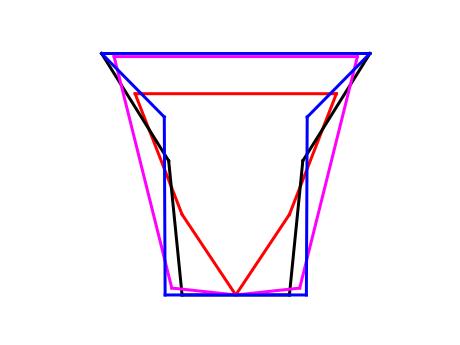
\includegraphics[width=2.3in]{figures/best_5_5_joint.png}
\end{center}
\caption{Best peg-socket joint (green and black) and initial peg-socket joint (red and blue) with five peg points and five socket edge. }
\label{fig:best_5_5_joint}
\end{figure}

For five-point and five-edge peg-socket joint, we get best joint from initial joint as shown in Figure~\ref{fig:best_5_5_joint}, which can be captured and has mininal maximum rotation angle but not break the insertion.

Figure~\ref{fig:best_5_5_sink} shows two sinks of best five-point and five-edge peg-in-socket motion graph. 

\begin{figure}
\begin{center}
\begin{subfigure}[t]{0.24\textwidth}
\begin{center}
\includegraphics[height=1.3in]{figures/best_5_5_sink1.png}
\end{center}
\label{fig:best_5_5_sink1}
\caption{Sink1. Contact mode with three contact pairs, e.g, ${cp}$ 1-1, ${cp}$ 3-3, ${cp}$ 4-4. }
\end{subfigure}
\begin{subfigure}[t]{0.24\textwidth}
\begin{center}
\includegraphics[height=1.3in]{figures/best_5_5_sink2.png}
\end{center}
\label{fig:best_5_5_sink2}
\caption{Sink2. Contact mode with three contact pairs, e.g, ${cp}$ 2-2, ${cp}$ 3-3, ${cp}$ 5-5. }
\end{subfigure}
\label{fig:best_5_5_sink}
\caption{Sinks of best peg-socket joint with five peg points and five socket edge. }
\end{center}
\end{figure}

